\chapter{Optimization using steepest descent method}
The reason SMT was selected for the purposes
of this thesis, was its ability to calculate
the derivatives of the trained  model. This 
ability makes the adjoint method 
unnecessary, since  the derivatives of
the objective function can now be 
approximated with the use of the surrogate 
model. This signifacantly reduced the 
computational cost of the optimization and 
enables the use of the ,otherly costly, 
steepest descent method. Steepest descent
is a first-order iterative optimization 
algorithm for finding a local minimum of a 
differentiable function. To find a local 
minimum of a function using gradient descent, 
steps proportional to the negative of 
the gradient (or approximate gradient) of the 
function at the current point are taken or in the form of 
a mathematical equation:

\begin{equation}\label{steepest descent}
	b^{n+1} = b^n - \eta \nabla F(b^n)
\end{equation}

where n the number of iterations and $\eta$ 
the step size, which is set constant
and equal to $\eta = 0.1$. The starting 
points b are manually inserted by the user 
and their compliance to the regarded 
boundaries is tested.
\\
  
The surrogate models used for the 
prediction of the partial derivatives are the 
KPLSK and QP. Moreover, since a discrete 
range of acceptable output values is only 
available for the the first objective 
function (\ref{3 design variable}), the 
testing will be focused on that 
equation.
\newpage
%-----------------------------------------------

\section{3 design variable equation}
The number of training points for the 
following tests is increased to $nt = 150$ 
for better model adaptation.
\\
\begin{itemize}
  \item \textbf{KPLSK}  
\begin{figure}[h]
    \centering
    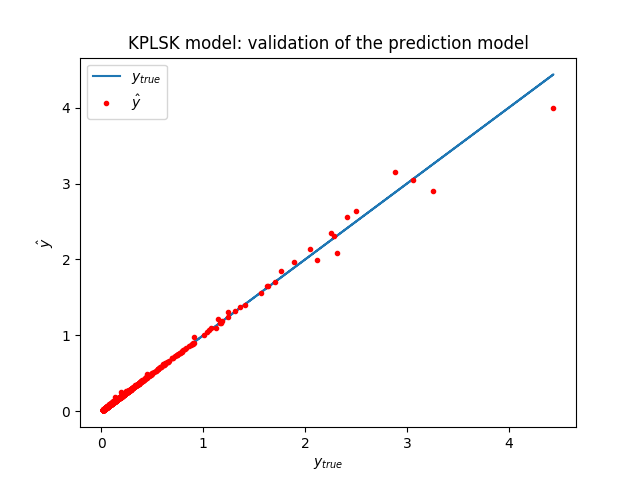
\includegraphics[width=0.7\textwidth]
    {Figure_21}
    \caption{KPLSK trained model for 800 
    validation 
    points, error : 0.0580883}
\end{figure} 
\\
\begin{figure}[h]
    \centering
    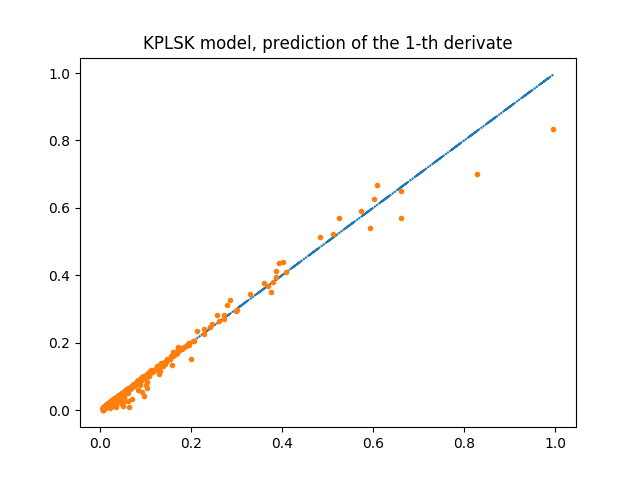
\includegraphics[width=0.7\textwidth]{Figure_22}
    \caption{Prediction of the 1st partial derivative 
    using KPLSK model, error: 0.0981615083}
\end{figure}  
\newpage
%------------------------------------------------------

\begin{figure}[H]
    \centering
    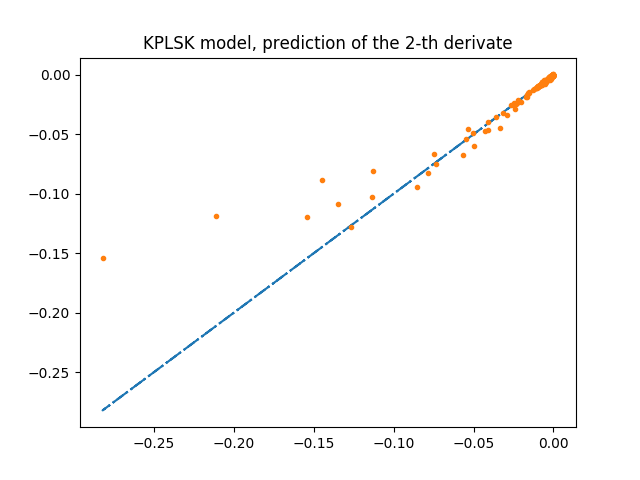
\includegraphics[width=0.9\textwidth]
    {Figure_23}
    \caption{Prediction of the 2nd partial 
    derivative 
    using KPLSK model, error: 0.332435532}
\end{figure} 

\begin{figure}[h]
    \centering
    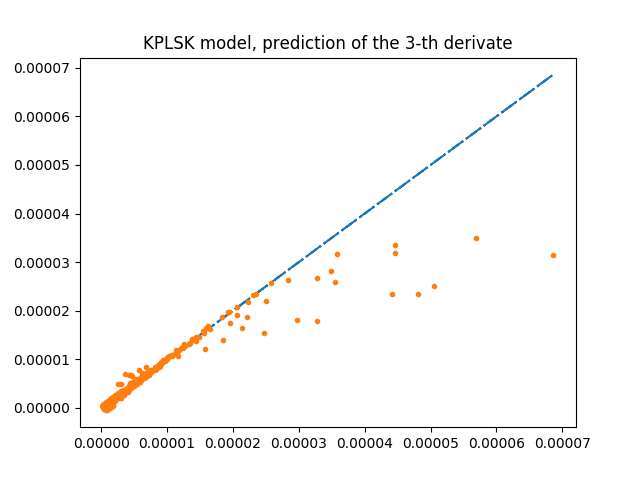
\includegraphics[width=0.9\textwidth]
    {Figure_24}
    \caption{Prediction of the 3rd partial 
    derivative 
    using KPLSK model, error 0.31252637}
\end{figure} 
\end{itemize}
\newpage
%-----------------------------------------------

The python script used for the prediction of
the partial derivatives calls the trained 
model using the .pickle() module. Then the 
SMT function $.predict\_derivatives()$ is 
called as such:
\begin{figure}[h]
    \centering
    \includegraphics[width=0.9\textwidth]{Figure_35}
    \caption{Prediction of F derivatives}
\end{figure}

Then the user must decide if they are 
satisfied with the predicted derivatives. If 
so, they are asked to insert a set of 
numeric values equal to the number of design
variables. Subsequently, it is tested if the
given values are located within the initial 
boundaries  set for each design variable. The 
final section consists from the steepest 
descent algorithm and when finished the 
process is repeated until the calculated 
mimimum objective function value is 
satisfactory. The described process is 
depicted in the following figure:  
 
\begin{figure}[h]
    \centering
    \includegraphics[width=0.9\textwidth]
    {Figure_25}
    \caption{Minimum objective 
    function value 
    	0.40599752}
\end{figure} 
\newpage
%----------------------------------------------

\begin{itemize}
  \item \textbf{QP}
\end{itemize}

	\begin{figure}[H]
    	\centering
    	\includegraphics[width=0.9\textwidth]
    	{Figure_26}\\ 
    	\caption{QP trained model for 800 validation 
    	points, error : 0.4533645183}
	\end{figure} 

\begin{figure}[h]
    \centering
    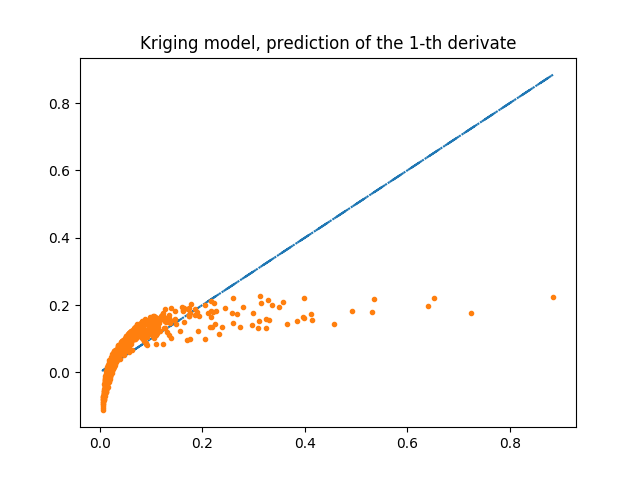
\includegraphics[width=0.85\textwidth]{Figure_27}\\
    \caption{Prediction of the 1st partial derivative 
    using QP model, error: 0.6003123463}
\end{figure}  
\newpage
%-----------------------------------------------------

\begin{figure}[h]
    \centering
    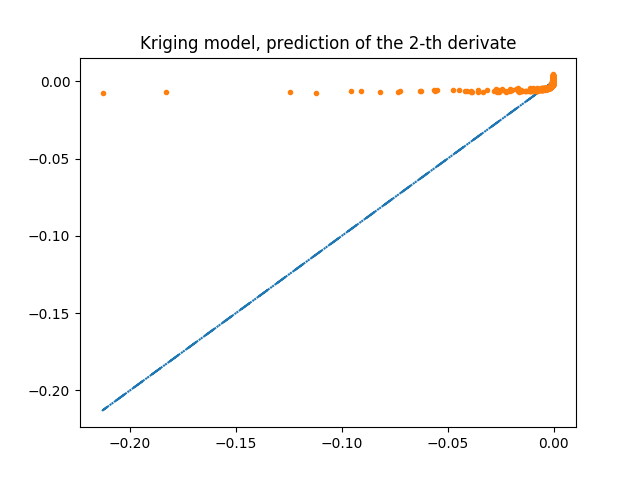
\includegraphics[width=0.9\textwidth]{Figure_28}\\
    \caption{Prediction of the 2nd partial derivative 
    using QP model, error: 0.920770299}
\end{figure} 

\begin{figure}[H]
    \centering
    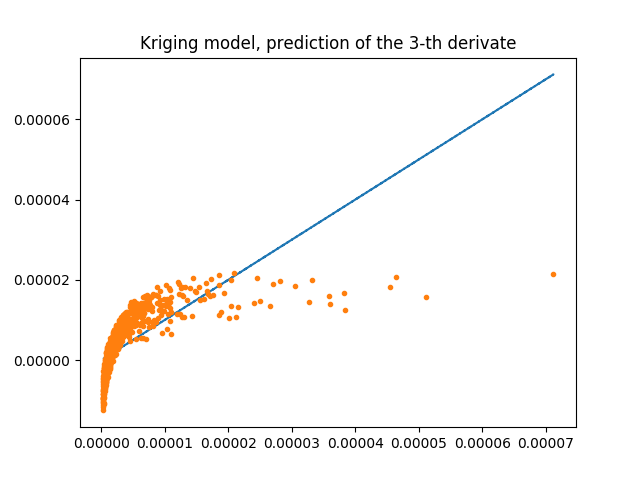
\includegraphics[width=0.9\textwidth]{Figure_29}\\
    \caption{Prediction of the 3rd partial derivative 
    using QP model, error 0.744598745}
\end{figure}  
\newpage
%----------------------------------------------------

Repeating the same process for the calculation of the
minimum of the objective function, using the QP model,
the following result occurs :
\begin{figure}[h]
    \centering
    \includegraphics[width=0.9\textwidth]{Figure_30}
    \caption{Minimum objective function value 
    	0.383112184}
\end{figure}  


\section{Observations}

QP minimizes the objective function better, due to
the fact that the steepest descent algorithm compares 
the user's inputs with the closest available value in 
the surrogates model dataset. Consequently, with $\eta$
constant, a better dataset can result in a better 
optimization regardless of the accuracy of the trained 
model. However, if the step size is variable 
as described by the $Barzilai - Borwein$ method :
\\
\begin{equation}
	\eta = \frac{\left| \left(x_{n} -x_{n-1}
    \right)^{T}  \left[ \nabla F(x_{n}) - 
    \nabla F(x_{n-1}) \right] \right|}
	{\left\| \nabla F(x_{n}) - \nabla F(x_{n-1})
	 \right\|^2}
\end{equation}
\\
then the accuracy of the surrogate model affects the 
result of the optimization. 

Moreover, with the completion of the second phase it 
becomes apparent that KPLSK is the most suitable 
surrogate model. In case the training is time-consuming
KPLSK can be replaced with KPLS, since they have small
differences.

Finally, the accuracy of the optimization process 
depends on the starting point provided by the user,
since \textbf{the steepest descent algorithm calculates 
the local minimum of the objective function in the 
vicinity of that point}. Consequently, with the same 
starting point a differently trained model can result 
in a lower local minimum , but a higher global mimimum.